\documentclass[mathserif]{beamer}
\usepackage{amsmath}
\usepackage{verbatim}
\usepackage{amsfonts}
\usepackage{color}
\usepackage{tgheros}
\useinnertheme{circles}
\setbeamertemplate{sidebar right}{}
\setbeamertemplate{footline}{%
\hfill\usebeamertemplate***{navigation symbols}
\hspace{0.2cm}\textcolor{red!39.22!green!58.43!blue!92.94!}{\insertframenumber{}/\inserttotalframenumber}}
%% 
\usepackage{lipsum}

\newcommand\blfootnote[1]{%
  \begingroup
  \renewcommand\thefootnote{}\footnote{#1}%
  \addtocounter{footnote}{-1}%
  \endgroup
}
\title{} 
\date{} 
\author{}

\begin{document}

\begin{frame}
 \frametitle{A fine mesh}
 \begin{figure}
  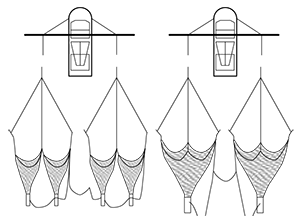
\includegraphics[width = 3in]{figures/quad_rig.png}
 \end{figure}
 \begin{figure}
  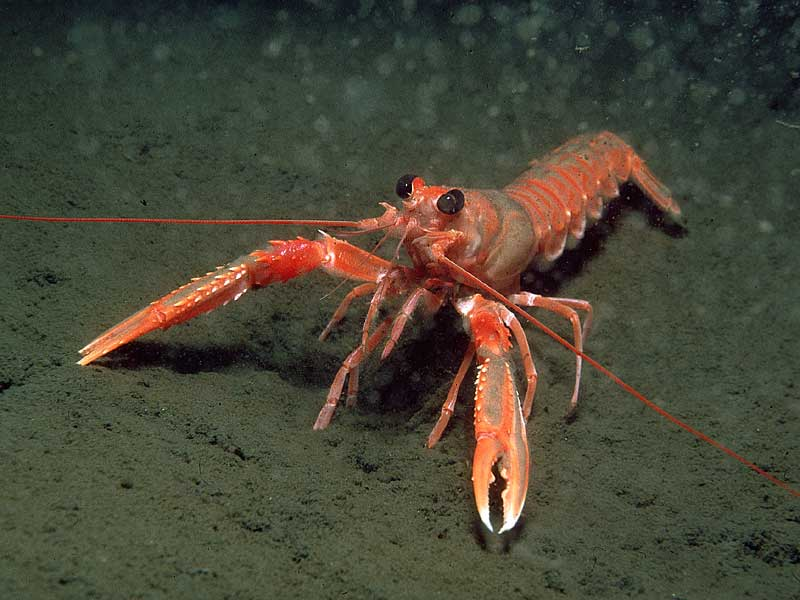
\includegraphics[width = 1.25in]{figures/nepnor.jpg}
 \end{figure}
\end{frame}

\begin{frame}
 \frametitle{The data}
 \begin{figure}
  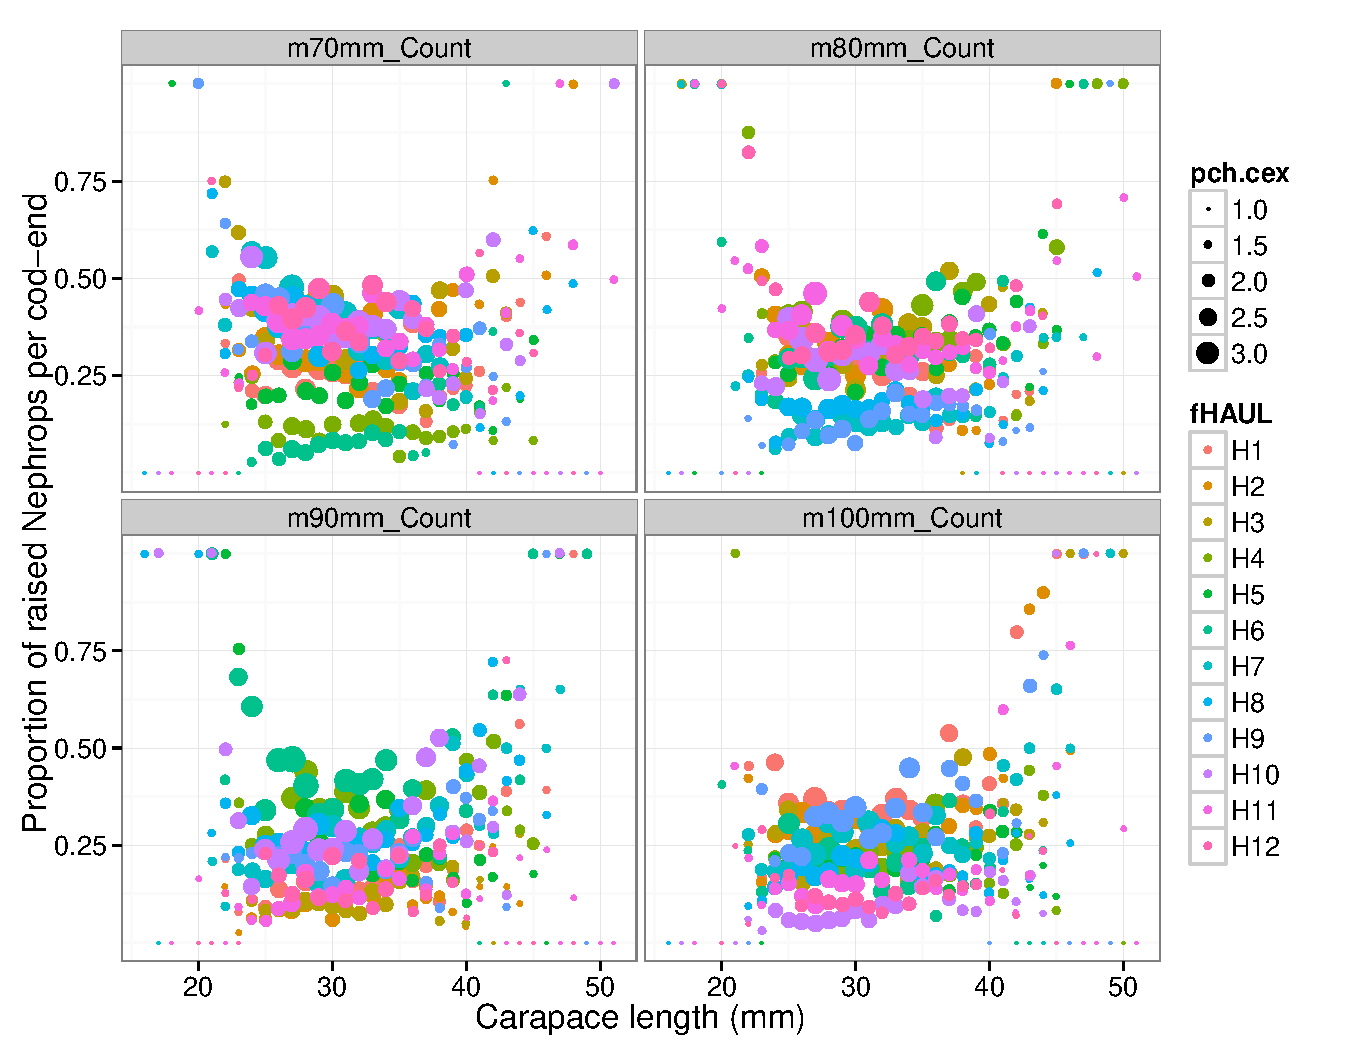
\includegraphics[width = 4in]{figures/bubble_gum_plots.pdf}
 \end{figure}
\end{frame}

\begin{frame}
 \frametitle{The model}
 \begin{equation*}
  P(Y_i = j) = \frac{e^{\mathbf{X}_i \boldsymbol{\beta}_j + \mathbf{u}_i}}{\sum_{k=1}^4 e^{\mathbf{X}_i \boldsymbol{\beta}_k + \mathbf{u}_i}} \blfootnote{Setting: $\boldsymbol{\beta}_{*,1} = 0$, $\mathbf{u}_{*,1} = 0$}
 \end{equation*}

  \begin{equation*}
  \mathbf{u}_{*,\{2,3,4\}} \sim \textnormal{N}_3(\mathbf{0}, \boldsymbol{\Sigma})
 \end{equation*}

 \end{frame}


\end{document}

